\documentclass[tikz]{standalone}
\usepackage{sourcecodepro}
\usetikzlibrary{arrows.meta,decorations.pathreplacing}

\begin{document}
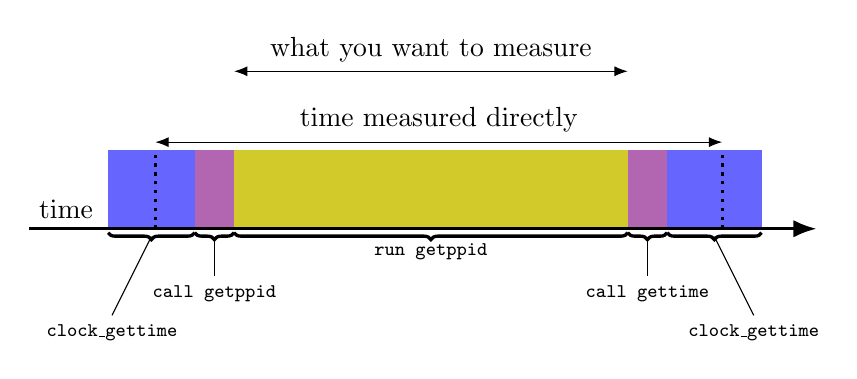
\begin{tikzpicture}
\fill[blue!60] (1, 0) rectangle ++(1.1, 1);
\fill[violet!60] (2.1, 0) rectangle ++(.5, 1);
\fill[yellow!80!black] (2.6, 0) rectangle ++(5, 1);
\fill[violet!60] (7.6, 0) rectangle ++(.5, 1);
\fill[blue!60] (8.1, 0) rectangle ++(1.2, 1);
\draw[very thick,-Latex] (0, 0.0) -- ++(10, 0.0);
\node[anchor=south west] at (0, 0.0) {time};

\draw[black,very thick,decorate,decoration={brace, mirror}] (1, -.05) -- ++(1.1, 0);
\draw (1.55, -.1) -- ++(-.5,-1) node[below,font=\tt\fontsize{7}{8}\selectfont]{clock\_gettime};
\draw[black,very thick,decorate,decoration={brace, mirror}] (2.1, -.05) -- ++(.5, 0);
\draw (2.35, -0.1) -- ++(0, -0.5)
    node[below,font=\tt\fontsize{7}{8}\selectfont]{call getppid};
\draw[black,very thick,decorate,decoration={brace, mirror}] (2.6, -.05) -- ++(5, 0)
    node[below,midway,font=\tt\fontsize{7}{8}\selectfont]{run getppid};
\draw[black,very thick,decorate,decoration={brace, mirror}] (7.6, -.05) -- ++(.5, 0);
\draw (7.85, -.1) -- ++(0, -0.5)
    node[below,font=\tt\fontsize{7}{8}\selectfont]{call gettime};
\draw[black,very thick,decorate,decoration={brace, mirror}] (8.1, -.05) -- ++(1.2, 0);
\draw (8.7, -.1) -- ++(.5,-1) node[below,font=\tt\fontsize{7}{8}\selectfont]{clock\_gettime};

\draw[Latex-Latex] (1.6, 1.1) -- (8.8, 1.1) node[above,midway] {time measured directly};
\draw[black,dotted,very thick] (1.6, 0) -- ++(0, 1);
\draw[black,dotted,very thick] (8.8, 0) -- ++(0, 1);
\draw[Latex-Latex] (2.6, 2.0) -- (7.6, 2.0) node[above,midway] {what you want to measure};

\end{tikzpicture}
\end{document}
